% ====================================================================
% Capítulo 6: Fluidos granulares
% ====================================================================
\chapter{El efecto Mpemba en fluidos granulares y gases de Maxwell}
\label{ch:granular}

\section{Motivación: disipación y desviación de la maxwelliana}

Los fluidos granulares ---suspensiones macroscópicas de partículas inelásticas, 
como arena, gránulos de polietileno o gránulos de azúcar--- constituyen el 
primer sistema fuera del agua donde el efecto Mpemba ha sido analítica y 
numéricamente demostrado de manera robusta. Lasanta, Vega Reyes, Prados y 
Santos~\cite{lasanta2017} probaron en 2017 que el fenómeno surge naturalmente del 
\emph{acoplamiento entre la temperatura granular y la curtosis de la 
distribución de velocidades}, sin necesidad de mecanismos extrínsecos.

\section{Termodinámica de un gas granular}

\subsection{Temperatura granular y distribución de Maxwell-Boltzmann}

Considérese un gas de $N$ esferas duras inelásticas en dimensión $d$, cada una 
con masa $m$, radio $a$ y coeficiente de restitución $\alpha \in (0, 1]$ 
(con $\alpha = 1$ correspondiendo al caso elástico). La \emph{temperatura 
granular} se define en términos de la energía cinética media:
\begin{equation}
    \frac{d}{2} n \kB T(t) = \frac{m}{2} \int \dd[d]{v} v^{2} f(\vb{v},t),
    \label{eq:granular_temp}
\end{equation}
%
donde $n$ es la densidad numérica y $f(\vb{v},t)$ es la función de distribución 
de velocidades, normalizada como $\int \dd[d]{v} f(\vb{v},t) = n$.

\subsection{Coeficiente de Sonine}

Para gases granulares, la distribución $f(\vb{v},t)$ típicamente \emph{no es 
maxwelliana} debido a la disipación inelástica. Se expande en polinomios de 
Sonine:
\begin{equation}
    f(\vb{v},t) = f_{M}(\vb{v},t) \, \left[1 + a_{2}(t) S_{2}(c^{2}) + a_{3}(t) S_{3}(c^{2}) + \cdots\right],
\end{equation}
%
donde $f_{M}$ es la maxwelliana, $\vb{c} = \vb{v}/v_{T}$ con $v_{T} = \sqrt{2 \kB T/m}$, 
y $S_{n}$ son los polinomios de Sonine. El coeficiente $a_{2}(t)$ representa la 
\emph{curtosis en exceso} y satisface
\begin{equation}
    a_{2}(t) = \frac{\langle v^{4} \rangle}{\frac{d+2}{d}\langle v^{2} \rangle^{2}} - 1.
    \label{eq:a2_kurtosis}
\end{equation}
%
\noindent En equilibrio (maxwelliano), $a_2 = 0$. Las colisiones inelásticas 
generan un valor asintótico no nulo $a_2^{\mathrm{HCS}}$ (estado de cooling 
homogéneo, \emph{homogeneous cooling state}).

\section{Ecuaciones de momentos truncadas}

A nivel de truncamiento de Sonine $a_3 = 0$, las ecuaciones de evolución son
\begin{equation}
\begin{aligned}
    \dv{T}{t} &= -\zeta(a_2, \alpha) \, T^{3/2}, \\
    \dv{a_2}{t} &= -\lambda_{a}(\alpha) \left[a_2 - a_2^{\mathrm{HCS}}(\alpha)\right] \, T^{1/2},
\end{aligned}
\label{eq:granular_moments}
\end{equation}
%
donde la tasa de enfriamiento $\zeta(a_2, \alpha)$ a primer orden en $1 - \alpha^2$ es
\begin{equation}
    \zeta(a_2, \alpha) = \frac{8}{3d} \sqrt{2\pi} \, (1 - \alpha^2) \left(1 + \frac{3 a_2}{16}\right).
    \label{eq:zeta}
\end{equation}
%
El valor estacionario de la curtosis, $a_2^{\mathrm{HCS}}$, es:
\begin{equation}
    a_2^{\mathrm{HCS}}(\alpha) = \frac{16 (1-\alpha)(1-2\alpha^2)}
    {57 - 25\alpha + 30 \alpha^2 (1-\alpha)}.
    \label{eq:a2_HCS}
\end{equation}
%
\noindent Por ejemplo, para $\alpha = 0.9$, $d = 3$: $a_2^{\mathrm{HCS}} \approx -0.027$.

\section{Argumento del efecto Mpemba granular}

La clave del efecto Mpemba en este sistema reside en el \emph{acoplamiento} 
entre $T$ y $a_2$: la tasa de enfriamiento $\zeta$ depende de $a_2$, de modo 
que dos preparaciones con la misma temperatura inicial pero diferente curtosis 
inicial enfriarán a tasas diferentes.

\subsection{Protocolo de Lasanta \emph{et al.}: dos preparaciones cruzadas}

\begin{itemize}
\item \textbf{Preparación A:} $T_A(0) = 1.0$, $a_2^{A}(0) = +0.5$ (curtosis positiva 
$\to$ distribución con colas pesadas; el sistema tiene partículas con velocidades 
extremas).
\item \textbf{Preparación B:} $T_B(0) = 0.99$, $a_2^{B}(0) = -0.35$ (curtosis 
negativa $\to$ distribución más estrecha que la maxwelliana).
\end{itemize}

\noindent A pesar de que $T_A(0) > T_B(0)$, el sistema $A$ enfría más rápido 
porque su mayor curtosis positiva incrementa $\zeta$ y por tanto la velocidad de 
transferencia de energía al exterior. El cruzamiento ocurre típicamente a 
$t^{\ast} \sim 0.2$ unidades de tiempo natural.

\subsection{Solución analítica y verificación numérica}

La integración de \cref{eq:granular_moments} mediante RK4 con $\alpha = 0.9$, 
$d = 3$ y los parámetros anteriores produce el cruzamiento de $T_A(t)$ y $T_B(t)$ 
en $t^{\ast} \approx 0.18$, con ambas trayectorias convergiendo al HCS 
$a_2 \to -0.027$.

\section{Simulación DSMC: Bird's algorithm}

Para validar las ecuaciones de momentos truncadas, se emplea el método de 
\emph{Direct Simulation Monte Carlo} (DSMC) de Bird~\cite{bird1994} para 
simular el sistema de partículas inelásticas. El algoritmo procede por pasos 
temporales discretos $\Delta t$:

\begin{enumerate}
\item \textbf{Movimiento balístico}: cada partícula recibe un avance 
$\vb{r}_i \to \vb{r}_i + \vb{v}_i \Delta t$.
\item \textbf{Selección de pares de colisión}: se muestrean $N_{\mathrm{coll}}$ 
pares aleatorios, con $N_{\mathrm{coll}} \propto N^2 \Delta t \nu$ y 
$\nu$ la frecuencia de colisión.
\item \textbf{Aceptación-rechazo}: cada par se acepta con probabilidad 
$\propto \abs{\vb{v}_i - \vb{v}_j} / \abs{\vb{v}_{\mathrm{rel,max}}}$ (No-Time 
Counter, NTC).
\item \textbf{Aplicación de regla inelástica}: para una colisión aceptada, las 
velocidades se actualizan según
\begin{equation}
    \vb{v}_i' = \vb{v}_i - \tfrac{1+\alpha}{2} (\vb{v}_{\mathrm{rel}} \cdot \hat{\vb{n}}) \hat{\vb{n}}, 
    \quad 
    \vb{v}_j' = \vb{v}_j + \tfrac{1+\alpha}{2} (\vb{v}_{\mathrm{rel}} \cdot \hat{\vb{n}}) \hat{\vb{n}},
    \label{eq:inelastic_collision}
\end{equation}
donde $\hat{\vb{n}}$ es un vector unitario aleatorio (en el caso de gases 
homogéneos sin gradientes espaciales).
\end{enumerate}

\subsection{Inicialización con curtosis deseada}

Una sutileza importante del protocolo de Lasanta \emph{et al.} es la 
\emph{preparación de las condiciones iniciales} con valores específicos de $T(0)$ 
y $a_2(0)$. Esto requiere generar una distribución de velocidades de la forma
\begin{equation}
    f(\vb{v}, 0) = f_{M}(v; T(0)) \left[1 + a_2(0) S_2(c^2)\right]
\end{equation}
%
mediante muestreo por rechazo o transformación de variables.

\section{Extensión a mezclas binarias: Biswas \emph{et al.}}

Biswas, Prasad, Raz y Rajesh~\cite{biswas2020} extendieron el formalismo a 
\emph{mezclas binarias de gases de Maxwell} sometidas a fuerzas externas 
(\emph{driven binary mixtures}). En este sistema, las especies $A$ y $B$ pueden 
tener masas $m_A, m_B$ y coeficientes de restitución $\alpha_{AA}, \alpha_{BB}, \alpha_{AB}$ 
diferentes.

\subsection{Acoplamiento difusión-colisión}

La ecuación de Boltzmann para cada especie es
\begin{equation}
    \pdv{f_s}{t} + \vb{a}_{s} \cdot \nabla_{\vb{v}} f_s = \sum_{s'} J_{ss'}[f_s, f_{s'}],
\end{equation}
%
donde $\vb{a}_s$ es la aceleración externa aplicada y $J_{ss'}$ es el operador 
de colisión inelástica entre especies. Los autores demuestran que el efecto 
Mpemba puede surgir de la \emph{diferencia} entre las tasas de difusión y 
colisión inter-especies cuando ambas se acoplan al campo externo.

\subsection{Aplicaciones a sistemas reales}

El formalismo de Biswas \emph{et al.} es aplicable a:
\begin{itemize}
\item Plasmas dustosos (mezclas de iones, electrones, partículas de polvo).
\item Mezclas de áridos en industria (\emph{mixing} en cementeras, silos).
\item Plasmas atómicos fríos (mezclas de isótopos enfriados por laser).
\end{itemize}

\section{Otras manifestaciones granulares: literatura adicional}

El paradigma granular del efecto Mpemba ha sido extendido a múltiples sistemas, 
todos referenciados en la revisión de Vu--Hayakawa~\cite{vuhayakawa2025}:

\begin{itemize}
\item Fluidos granulares con \textbf{forzamiento estocástico}: López-Castaño 
\emph{et al.} mostraron que la temperatura granular puede oscilar como respuesta 
a un ruido térmico aplicado al baño.
\item Mezclas asimétricas $A$-$B$ con \textbf{gradientes térmicos}: Gómez 
González, Khalil y Garzó~\cite{biswas2020} caracterizaron el efecto en flujos 
de cizalla.
\item Sistemas \textbf{cuasi-2D} sobre placas vibradas: experimentos con 
gránulos de polietileno mostraron el efecto en el régimen sub-amortiguado.
\end{itemize}

\section{Implementación numérica}

El módulo \texttt{mpemba\_granular\_analytic} de \texttt{Mpemba-X v2} integra las 
ecuaciones de momentos \cref{eq:granular_moments} mediante RK4 con 
$\Delta t = 10^{-3}$. La validación reproduce la Fig. 4 de Lasanta \emph{et 
al.}~\cite{lasanta2017} con cruzamiento $t^{\ast} \approx 0.18$.

El módulo complementario \texttt{mpemba\_granular\_dsmc} implementa el algoritmo 
DSMC con $N = 30000$ partículas en una caja con condiciones periódicas de 
contorno, paralelizado con OpenMP sobre el lazo de movimiento balístico y MPI 
sobre múltiples réplicas estadísticas. La curtosis se mide directamente como
\begin{equation}
    \hat{a}_2 = \frac{\langle v^4 \rangle}{\frac{d+2}{d} \langle v^2 \rangle^{2}} - 1,
\end{equation}
%
con promedio sobre el ensemble de partículas.

\begin{figure}[h]
\centering
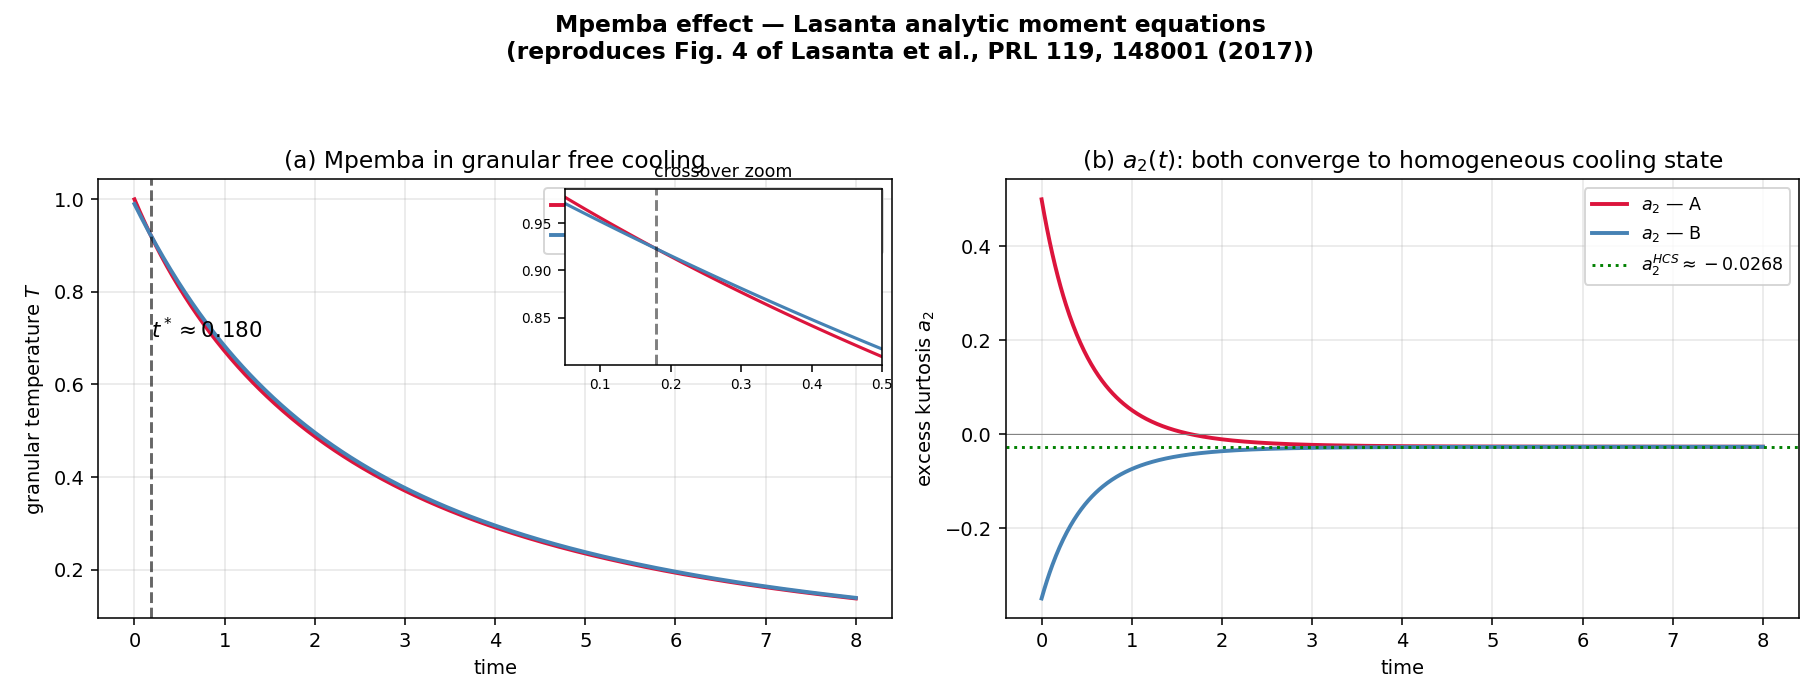
\includegraphics[width=0.95\textwidth]{figures/granular.png}
\caption{Reproducción de la Fig. 4 de Lasanta \emph{et al.} (2017) usando las 
ecuaciones de momentos del módulo \texttt{mpemba\_granular\_analytic}. 
Cruzamiento de $T(t)$ a $t^{\ast} \approx 0.18$ y convergencia de $a_2(t)$ al 
valor HCS $\approx -0.027$.}
\label{fig:granular_validation}
\end{figure}
